\documentclass[10pt]{beamer}

\usetheme{Madrid}
\usecolortheme{default}
\usepackage[utf8]{inputenc}
\usepackage{graphicx}
\usepackage{amsmath}
\usepackage{amssymb}
\usepackage{booktabs}
\usepackage{array}

\setbeamertemplate{navigation symbols}{}

\title[CTW for Real-Valued Time Series]{Context-Tree Weighting for Real-Valued Time Series}
\subtitle{Bayesian Inference with Hierarchical Mixture Models}
\author{Raphaël Faure - Max Defez - Tristan Beruard}
\date{April 2026}

\begin{document}

%--- Title slide
\begin{frame}
\titlepage
\end{frame}

%--- Outline
\begin{frame}{Outline}
\tableofcontents
\end{frame}

%%%%%%%%%%%%%%%%%%%%%%%%%%%%%%%%%%%%%%%%%%%%%%%%%%
\section{Project Overview}
%%%%%%%%%%%%%%%%%%%%%%%%%%%%%%%%%%%%%%%%%%%%%%%%%%

\begin{frame}{Project Overview}
\begin{block}{Objectives}
\begin{itemize}
    \item Implement the BCT-AR algorithm from the paper by Papageorgiou \& Kontoyiannis (2023)
    \item Extend the framework to a \textbf{bivariate} setting
    \item Evaluate performance against classical AR baselines on both synthetic and real datasets
\end{itemize}
\end{block}
\begin{block}{Models presented}
\begin{itemize}
    \item BCT-AR (Bayesian Context Tree AutoRegressive) --- Univariate
    \item BCT-AR --- Bivariate (two variants: V1 and V2)
\end{itemize}
\end{block}
\end{frame}

%%%%%%%%%%%%%%%%%%%%%%%%%%%%%%%%%%%%%%%%%%%%%%%%%%
\section{BCT-AR: Algorithm Description}
%%%%%%%%%%%%%%%%%%%%%%%%%%%%%%%%%%%%%%%%%%%%%%%%%%

\begin{frame}{BCT-AR: Prediction Objective and Quantisation}
\begin{itemize}
    \item \textbf{Prediction objective:} Consider a real-valued time series $(x_t)_{t\geq 1}$. We model
    \[
    p(x_t \mid x_{t-1}, x_{t-2}, \dots)
    \]
    for probabilistic forecasting.

    \item \textbf{Quantisation:} Introduce a quantiser $Q : \mathbb{R} \to \mathcal{A} = \{0,\dots,m-1\}$:
    \[
    Q(x)=
    \begin{cases}
    0, & x<c_1,\\
    i, & c_i \le x \le c_{i+1},\\
    m-1, & x>c_{m-1}.
    \end{cases}
    \]
    Maps real-valued observations to a finite alphabet.

    \item \textbf{Discrete context:} For maximum depth $D$, define the quantised past
    \[
    t_t = (Q(x_{t-1}), \dots, Q(x_{t-D}))
    \]
    encoding the recent history.
\end{itemize}
\end{frame}

\begin{frame}{BCT-AR: Context Tree and State Partition}
\begin{itemize}
    \item \textbf{Context tree:} A proper $m$-ary tree $T$ of depth at most $D$. The context $s_t$ of $x_t$ is the leaf of $T$ that is a suffix of $t_t$, allowing variable-length memory.

    \item \textbf{State partition:} The leaves $s \in T$ define a partition of past histories into \emph{regimes}, each with a different predictive behaviour.

    \item \textbf{General model (BCT-SSM):} A parametric model $M_s$ with parameters $\theta_s$ is assigned to each leaf. The likelihood factorises as
    \[
    p(x \mid T,\theta)
    =
    \prod_{s\in T} \prod_{i\in B_s}
    p(x_i \mid \theta_s, x_{i-1},\dots,x_{i-D}),
    \]
    where $B_s$ is the set of indices assigned to context $s$.
\end{itemize}
\end{frame}

\begin{frame}{BCT-AR: Bayesian Prior Structure}
\begin{itemize}
    \item \textbf{Tree prior:} A Bayesian prior is placed over trees:
    \[
    \pi(T)=\alpha^{|T|-1}\beta^{|T|-L_D(T)}, \quad \alpha=(1-\beta)^{1/(m-1)},
    \]
    penalising complex trees and controlling overfitting.

    \item \textbf{Parameter prior:} Conditional on $T$, parameters are independent across leaves:
    \[
    \pi(\theta \mid T)=\prod_{s\in T}\pi(\theta_s).
    \]

    \item \textbf{Evidence (marginal likelihood):}
    \[
    p(x)=
    \sum_{T} \pi(T) \int p(x \mid T,\theta)\pi(\theta \mid T)\,d\theta
    \]
    integrates over all trees and parameters.

    \item \textbf{Node marginal likelihood:} For each node $s$:
    \[
    P_e(s,x)=
    \int \prod_{i\in B_s} p(x_i \mid \theta_s)\pi(\theta_s)\,d\theta_s.
    \]
\end{itemize}
\end{frame}

\begin{frame}{BCT-AR: CCTW and CBCT Algorithms}
\begin{block}{CCTW recursion (evidence computation)}
\[
P_{w,s}=
\begin{cases}
P_e(s,x) & \text{(leaf)},\\
\beta P_e(s,x) + (1-\beta)\prod_{j=0}^{m-1}P_{w,sj} & \text{(otherwise)}.
\end{cases}
\]
At the root, $P_{w,\text{root}} = p(x)$ exactly.
\end{block}

\begin{block}{CBCT recursion (MAP tree)}
\[
P_{m,s}=
\max\left\{
\beta P_e(s,x),\;
(1-\beta)\prod_{j=0}^{m-1}P_{m,sj}
\right\}
\]
Produces the MAP tree $T^* = \arg\max_T\, p(T \mid x)$ via a pruning procedure.
\end{block}
\end{frame}

\begin{frame}{BCT-AR: The Autoregressive Leaf Model}
\begin{itemize}
    \item \textbf{BCT-AR model:} Each leaf uses an AR$(p)$ model:
    \[
    x_t = \phi_s^\top \tilde{x}_{t-1} + e_t, \quad e_t \sim \mathcal{N}(0,\sigma_s^2),\quad
    \tilde{x}_{t-1}=(x_{t-1},\dots,x_{t-p})^\top.
    \]
    Results in a nonlinear mixture of local linear models.

    \item \textbf{Conjugate priors:}
    \[
    \sigma_s^2 \sim \mathrm{Inv\text{-}Gamma}(\tau,\lambda), \quad
    \phi_s \mid \sigma_s^2 \sim \mathcal{N}(\mu_0,\sigma_s^2\Sigma_0).
    \]

    \item \textbf{Sufficient statistics:}
    \[
    s_1=\sum_{i\in B_s}x_i^2,\quad
    s_2=\sum_{i\in B_s}x_i \tilde{x}_{i-1},\quad
    S_3=\sum_{i\in B_s}\tilde{x}_{i-1}\tilde{x}_{i-1}^\top.
    \]
\end{itemize}
\end{frame}

\begin{frame}{BCT-AR: Closed-Form Posteriors and MAP Estimates}
\begin{itemize}
    \item \textbf{Integrated likelihood (closed form):}
    \[
    P_e(s,x)=
    C_s^{-1}
    \frac{\Gamma(\tau+|B_s|/2)\,\lambda^\tau}
    {\Gamma(\tau)\,(\lambda+D_s/2)^{\tau+|B_s|/2}}.
    \]

    \item \textbf{Posterior distributions:}
    \[
    \sigma_s^2 \mid T,x \sim \mathrm{Inv\text{-}Gamma}\!\left(\tau+\tfrac{|B_s|}{2},\; \lambda+\tfrac{D_s}{2}\right),
    \]
    \[
    \phi_s \mid T,x \sim t_\nu(m_s, P_s).
    \]

    \item \textbf{MAP estimates (used for prediction):}
    \[
    \hat{\phi}_s = m_s, \qquad
    \hat{\sigma}_s^2 = \frac{2\lambda+D_s}{2\tau+|B_s|+2}.
    \]

    \item \textbf{Sequential updates:} When a new observation arrives, only $D+1$ nodes need to be updated $\Rightarrow O(D)$ operations per step (i.e.\ $O(1)$ in $n$).
\end{itemize}
\end{frame}

%%%%%%%%%%%%%%%%%%%%%%%%%%%%%%%%%%%%%%%%%%%%%%%%%%
\section{BCT-AR Univariate: Implementation}
%%%%%%%%%%%%%%%%%%%%%%%%%%%%%%%%%%%%%%%%%%%%%%%%%%

\begin{frame}{Univariate BCT-AR: Implementation}
One \texttt{BCT-AR} class with two main methods:

\begin{block}{\texttt{observe(x)}}
\begin{enumerate}
    \item Quantise the past of $x$ up to max depth $\Rightarrow$ path in the tree.
    \item Traverse the tree along the path; update $\{|B_s|, s_1, s_2, S_3\}$ and $P_e(s,x)$. Update AR MAP parameters. \emph{(Complexity: linear in depth.)}
    \item Apply CCTW update: recursive update of $P_{w,s}$.
    \item Apply CBCT update: recursive update and pruning of $P_{m,s}$.
\end{enumerate}
\end{block}

\begin{block}{\texttt{predict(x)}}
\begin{enumerate}
    \item Quantise the context up to max depth $\Rightarrow$ path in the tree.
    \item Traverse the tree until a leaf is reached.
    \item Predict the next value using the leaf's MAP parameters.
\end{enumerate}
\end{block}

\textbf{Key advantages:} Captures nonlinear dependencies; computationally efficient.
\end{frame}

\begin{frame}{Univariate BCT-AR: Computational Efficiency}
Comparison with simple AR model from the \texttt{statsmodels} Python package.

\begin{figure}
    \centering
    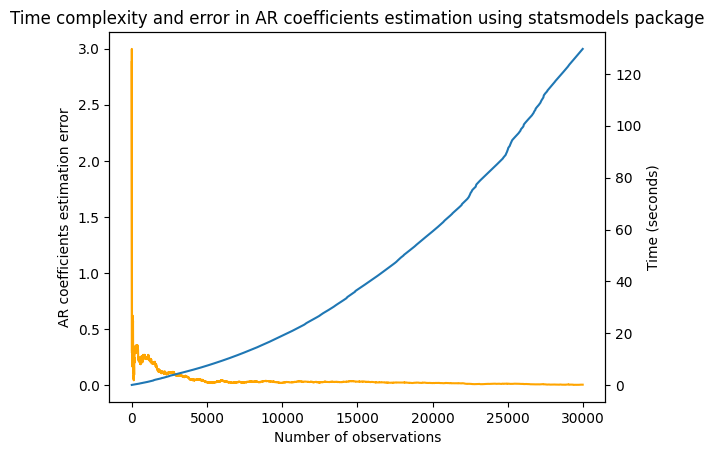
\includegraphics[width=0.75\textwidth]{complexity/statsmodel_complexity.png}
    \caption{Complexity: \texttt{statsmodels} AR model (sequential refitting)}
\end{figure}
\end{frame}

\begin{frame}{Univariate BCT-AR: Computational Efficiency (cont.)}
\begin{figure}
    \centering
    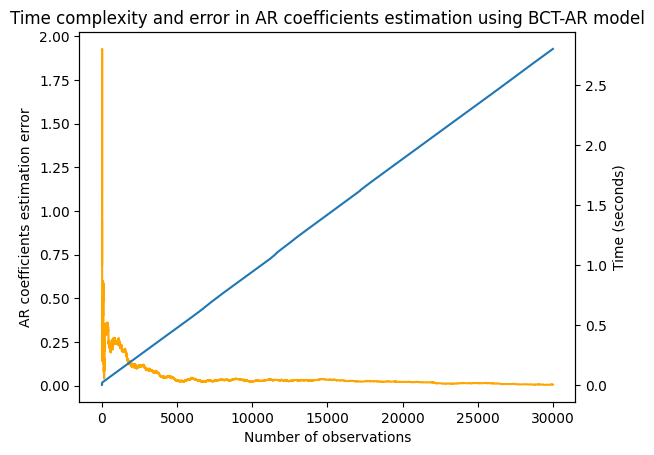
\includegraphics[width=0.75\textwidth]{complexity/bct_ar_complexity.png}
    \caption{Complexity: BCT-AR model (sequential update)}
\end{figure}
The BCT-AR model supports efficient online updates, unlike standard AR refitting.
\end{frame}

%%%%%%%%%%%%%%%%%%%%%%%%%%%%%%%%%%%%%%%%%%%%%%%%%%
\section{Univariate BCT-AR: Experiments}
%%%%%%%%%%%%%%%%%%%%%%%%%%%%%%%%%%%%%%%%%%%%%%%%%%

\begin{frame}{Univariate: Artificial Data --- Setup}
\begin{itemize}
    \item First tested on artificially generated data with increasing complexity.
    \item Simple AR(2) test:
    \[
    x_t = a\,x_{t-1} + b\,x_{t-2} + \sigma
    \]
    The algorithm trivially recovered the model, so we moved to harder settings.
\end{itemize}
\end{frame}

\begin{frame}{Univariate: Artificial Data --- AR Mixture}
We worked with AR(2) mixtures conditioned on the past of the variable:
\[
x_t =
\begin{cases}
a_1 x_{t-1} + b_1 x_{t-2} + \sigma_1 & \text{if } x_{t-1} < 0, \\
a_2 x_{t-1} + b_2 x_{t-2} + \sigma_2 & \text{if } x_{t-1} \geq 0.
\end{cases}
\]
\end{frame}

\begin{frame}{Univariate: Artificial Data --- Results}
Training on $20\,000$ data with
\[
a_1 = 0.5,\; b_1 = -0.3,\; \sigma_1 = 0.1,\; a_2 = -0.4,\; b_2 = 0.2,\; \sigma_2 = 0.2.
\]
\begin{figure}
    \centering
    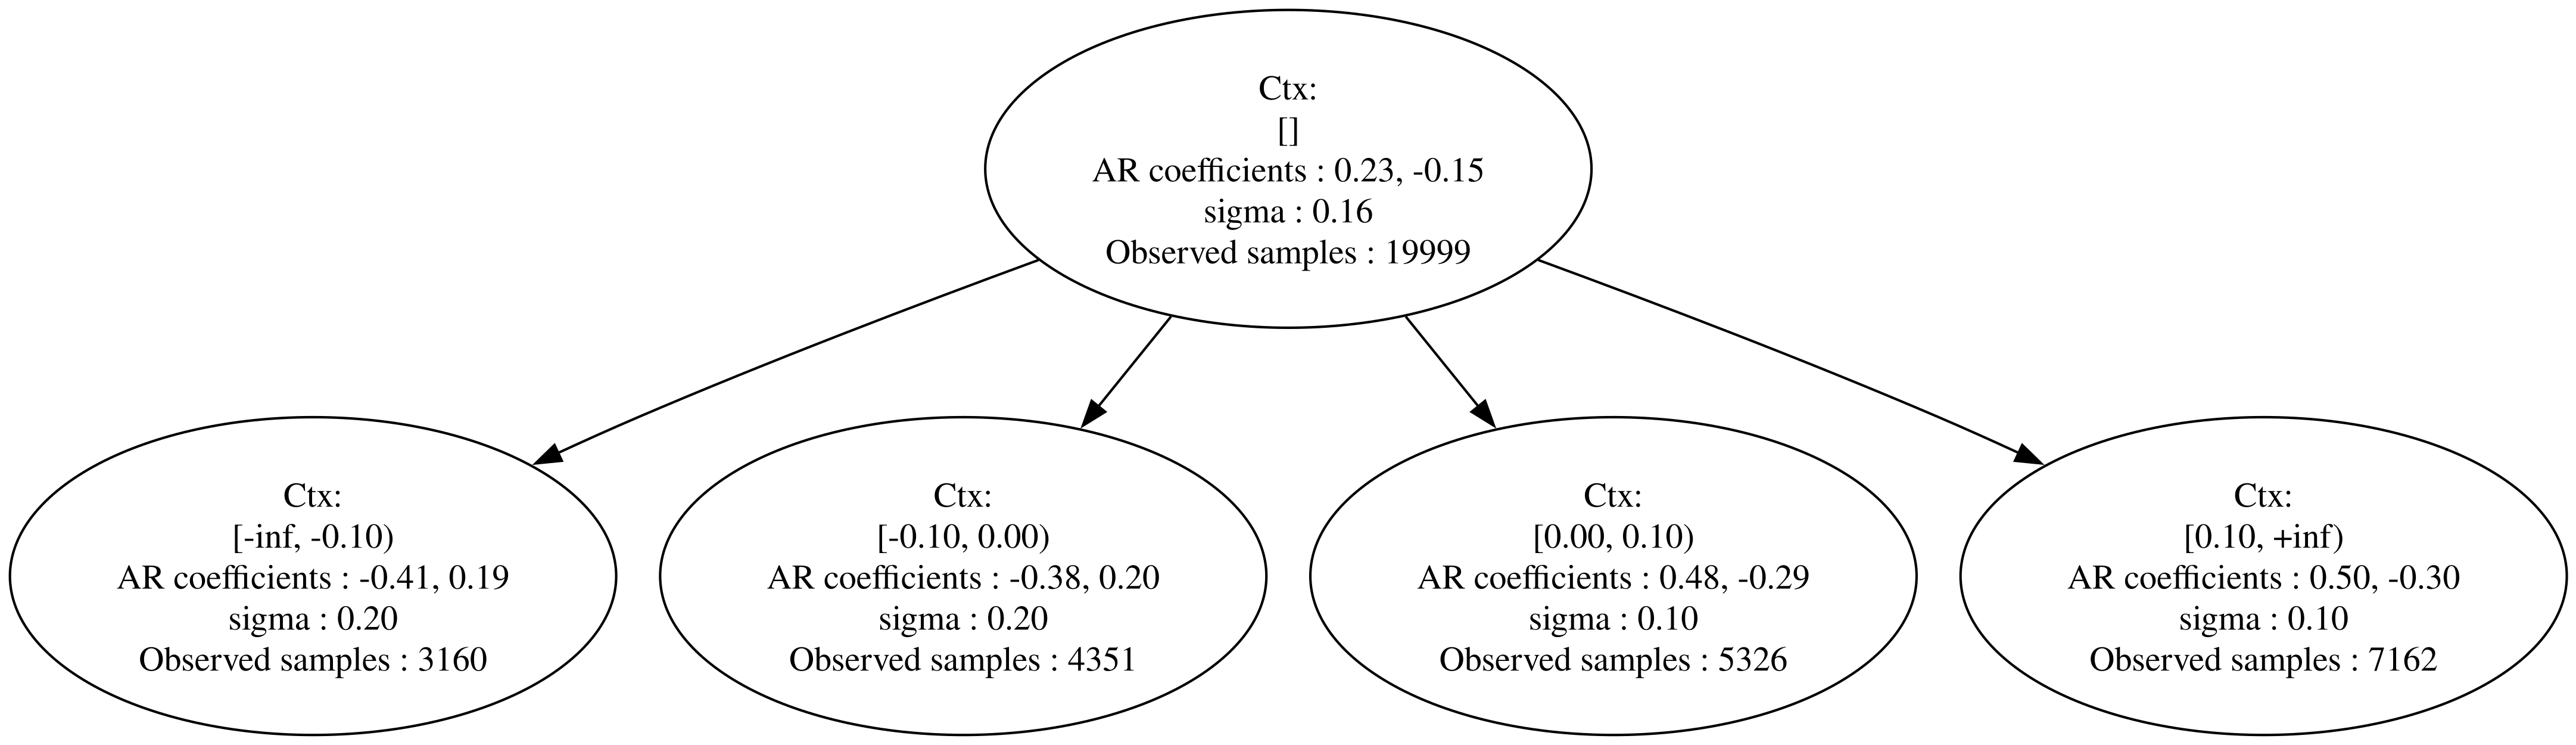
\includegraphics[width=0.78\textwidth]{artificial_data/univariate.png}
    \caption{Univariate tree for AR mixture}
\end{figure}
The algorithm correctly identifies the two regimes and prunes the tree to depth 1 (max depth was 3), understanding that older context is not relevant.
\end{frame}

\begin{frame}{Univariate: Sensitivity to Hyperparameters}
However, the model is sensitive to the number of training samples and $\beta$.

Setting the number of training samples to only $100$ leads to this underfitting (averaged) tree:

\begin{figure}
    \centering
    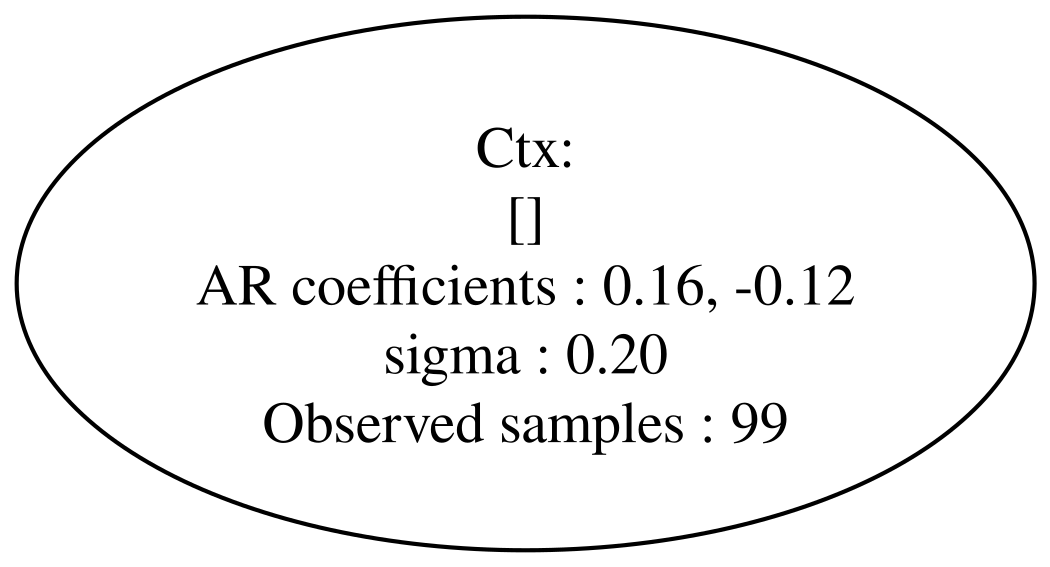
\includegraphics[width=0.78\textwidth]{artificial_data/univariate_overfit.png}
    \caption{Underfitting with univariate tree for AR mixture (100 samples)}
\end{figure}

\textbf{Conclusion:} Architecture performs well on shallow artificial data. Hyperparameter tuning is critical.
\end{frame}

\begin{frame}{Univariate: Real Data --- Unemployment Rate Dataset}
\begin{itemize}
    \item US unemployment rate from 1948 to 2018.
    \item Following the paper: work on the first-differenced series $\Delta x_t = x_t - x_{t-1}$.
    \item Threshold set at $0.15$ (splits nodes into $> 0.15$ and $\leq 0.15$).
    \item Dataset standardised.
\end{itemize}

\begin{figure}
    \centering
    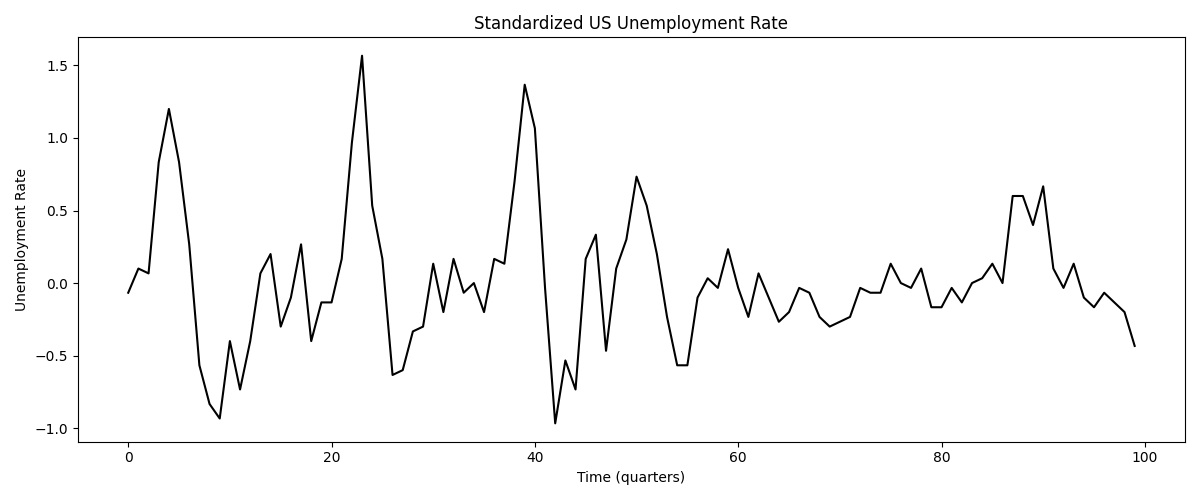
\includegraphics[width=0.78\textwidth]{UR/unemployment_rate_no_regimes.png}
    \caption{US unemployment rate (no regimes)}
\end{figure}
\end{frame}

\begin{frame}{Univariate: Real Data --- Fitted Tree}
\begin{figure}
    \centering
    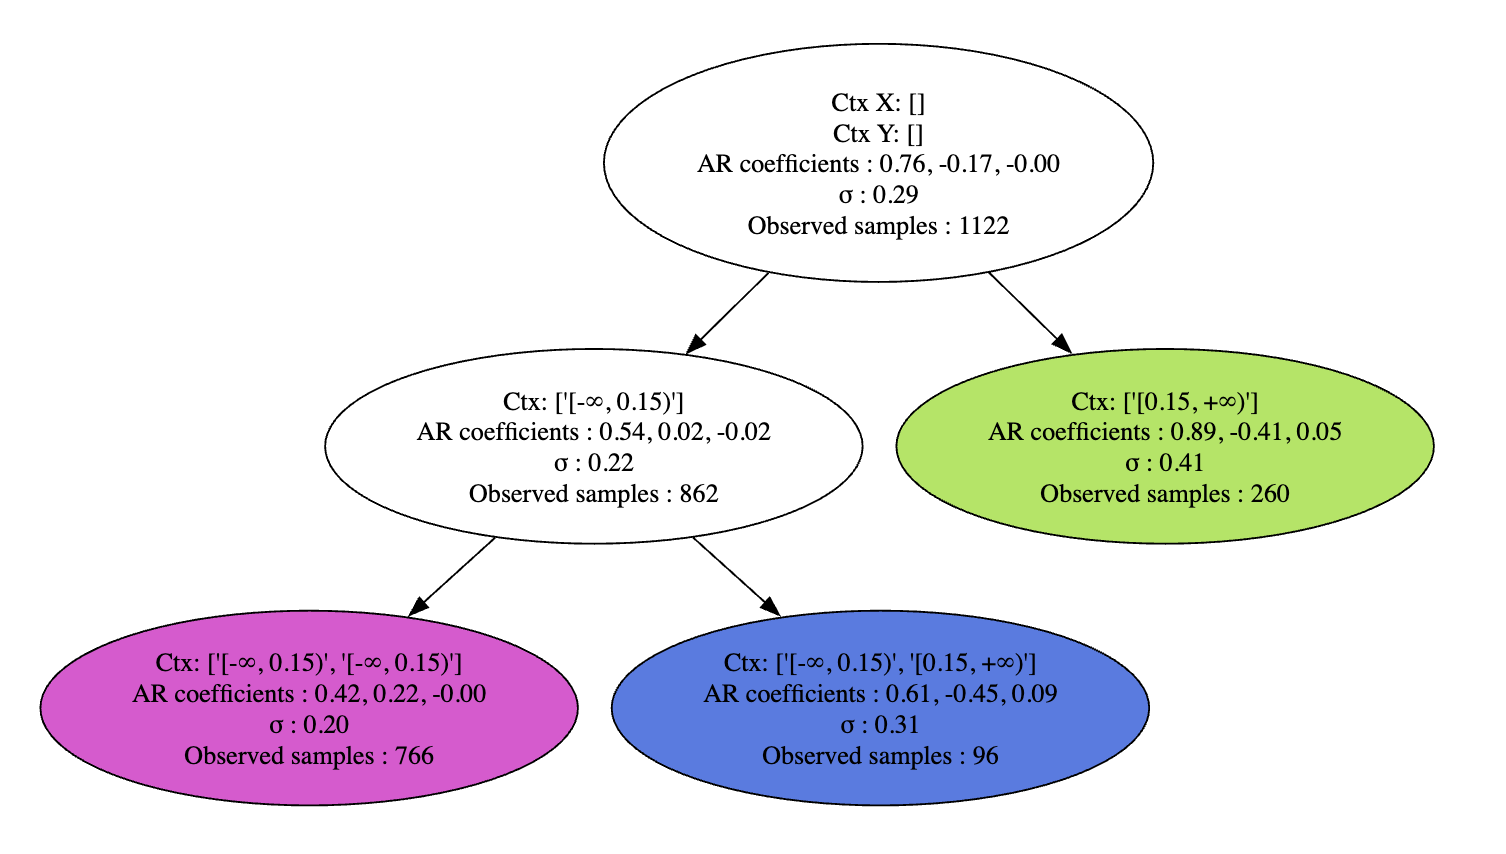
\includegraphics[width=0.75\textwidth]{UR/unemployment_tree.png}
    \caption{BCT-AR fitted tree on US unemployment rate}
\end{figure}
\end{frame}

\begin{frame}{Univariate: Real Data --- Regime Identification}
\begin{figure}
    \centering
    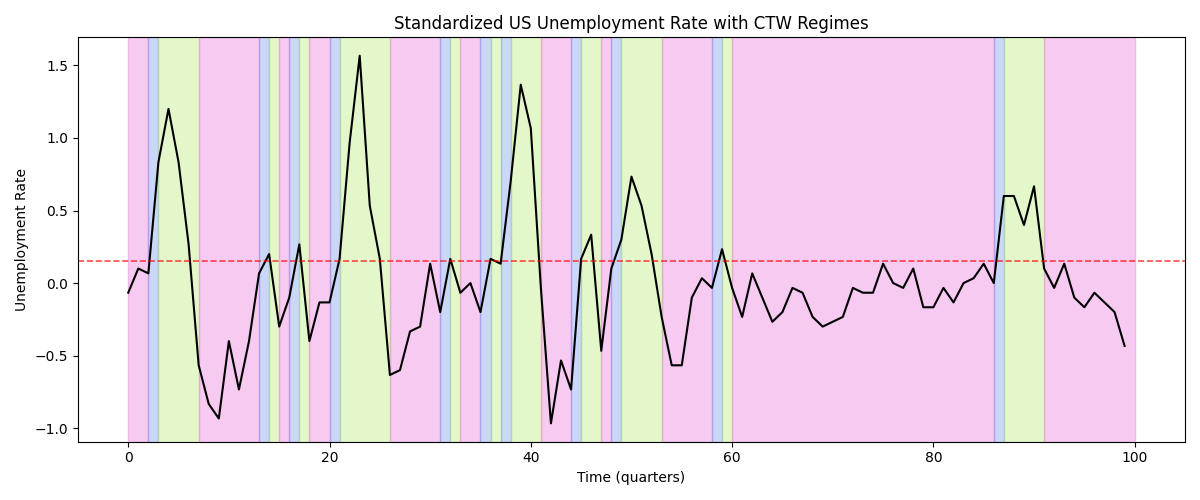
\includegraphics[width=0.78\textwidth]{UR/unemployment_rate.png}
    \caption{Unemployment rate with identified regimes over time}
\end{figure}
\end{frame}

\begin{frame}{Univariate: Real Data --- Forecasting Results}
1-step prediction results on the US unemployment rate dataset:

\begin{table}[h]
\centering
\begin{tabular}{lcc}
\toprule
Model & MSE & MAE \\
\midrule
Baseline (lag 1) & 0.10323 & 0.23618 \\
AR(2) & 0.08268 & 0.21389 \\
\textbf{CTW (BCT-AR)} & \textbf{0.07758} & \textbf{0.20355} \\
\bottomrule
\end{tabular}
\caption{1-step forecasting results on US unemployment rate}
\end{table}

\textbf{BCT-AR achieves the best performance on both MSE and MAE.}
\end{frame}

%%%%%%%%%%%%%%%%%%%%%%%%%%%%%%%%%%%%%%%%%%%%%%%%%%
\section{BCT-AR Bivariate: Algorithm Description}
%%%%%%%%%%%%%%%%%%%%%%%%%%%%%%%%%%%%%%%%%%%%%%%%%%

\begin{frame}{Bivariate BCT-AR: Motivation and Ideas}
\textbf{Idea:} Add additional data to the context to improve prediction (from intuition or correlated data).

\begin{block}{Bivariate V1}
Change the quantiser to quantise along two axes simultaneously at each level.\\
\textbf{Issues:} Very small slots per node (few observations), prone to overfitting.
\end{block}

\begin{block}{Bivariate V2}
Configured with a \emph{quantiser sequence} indicating the order of quantisation variables (e.g.\ $[1, 0, 0]$). Unidimensional quantisers are passed for each variable.
\begin{itemize}
    \item \textbf{Goal:} Allow splitting on $X$ more than on $Y$ --- each depth level corresponds to a split on a given variable.
    \item The tree depth penalisation naturally discourages over-splitting on $Y$.
\end{itemize}
\end{block}
\end{frame}

%%%%%%%%%%%%%%%%%%%%%%%%%%%%%%%%%%%%%%%%%%%%%%%%%%
\section{Bivariate BCT-AR: Experiments}
%%%%%%%%%%%%%%%%%%%%%%%%%%%%%%%%%%%%%%%%%%%%%%%%%%

\begin{frame}{Bivariate: Artificial Data --- Setup}
We generated a series $x$ from a mixture of AR models, conditioned on the value of another series $y$ (itself an AR process):

\begin{equation}
x_t =
\begin{cases}
a_1 x_{t-1} + b_1 x_{t-2} + \sigma_1 & \text{if } y_t < \theta_1, \\
a_2 x_{t-1} + b_2 x_{t-2} + \sigma_2 & \text{if } \theta_1 \le y_t < \theta_2, \\
a_3 x_{t-1} + b_3 x_{t-2} + \sigma_3 & \text{if } \theta_2 \le y_t < \theta_3, \\
a_4 x_{t-1} + b_4 x_{t-2} + \sigma_4 & \text{if } y_t \ge \theta_3.
\end{cases}
\end{equation}

\[
y_t = a y_{t-1} + b y_{t-2} + \sigma.
\]

Both bivariate models were trained on the same data with the same hyperparameter tuning procedure.
\end{frame}

\begin{frame}{Bivariate: Artificial Data --- Parameters and V1 Results}
Parameters:
\footnotesize
\[
\sigma_{1,2,3,4} = 0.05,\quad a_1{=}1,\; b_1{=}{-}0.5,\quad a_2{=}{-}0.8,\; b_2{=}0.7,\quad a_3{=}0.4,\; b_3{=}{-}0.7,
\]
\[
a_4{=}{-}0.5,\; b_4{=}0.4,\quad \theta_1{=}{-}0.05,\; \theta_2{=}0,\; \theta_3{=}0.05.
\]
\normalsize

\begin{figure}[h]
    \centering
    
\includegraphics[width=0.72\textwidth]{artificial_data/bivar_v1_tree.png}
    \caption{Bivariate tree (V1) for conditioned AR mixture}
\end{figure}
The model correctly identifies the coefficients and prunes unnecessary depth (max depth = 3).
\end{frame}

\begin{frame}{Bivariate: Artificial Data --- V2 Results}
\begin{figure}[h]
    \centering
    
\includegraphics[width=0.72\textwidth]{artificial_data/bivar_v2_tree.png}
    \caption{Bivariate tree (V2) for conditioned AR mixture}
\end{figure}
Different tree shape but consistent results: the model correctly identifies the underlying structure.
\end{frame}

\begin{frame}{Bivariate: Artificial Data --- Prediction Benchmark}
Prediction at horizon $k \geq 1$. High signal-to-noise ratio of AR models ($\approx 50\%$) makes long-horizon prediction difficult.

\begin{table}[h]
\centering
\small
\begin{tabular}{lcc}
\toprule
Model & MAE ($k=1$) & MAE ($k=10$) \\
\midrule
Baseline (lag 1) & $0.129 \pm 10^{-2}$ & $0.155 \pm 2{\times}10^{-2}$ \\
AR & $0.072 \pm 9{\times}10^{-3}$ & $0.090 \pm 8{\times}10^{-3}$ \\
Bivariate tree V1 & $0.068 \pm 9{\times}10^{-3}$ & $0.085 \pm 9{\times}10^{-3}$ \\
\textbf{Bivariate tree V2} & $\mathbf{0.064 \pm 8{\times}10^{-3}}$ & $0.092 \pm 8{\times}10^{-3}$ \\
\bottomrule
\end{tabular}
\caption{Benchmark on MAE for two prediction horizons $k$}
\end{table}

Bivariate trees outperform shallow baselines; improvement over AR is modest at longer horizons due to noise.
\end{frame}

\begin{frame}{Bivariate: Artificial Data --- Transition to Real Data}
\textbf{Conclusion on artificial data:} Both architectures perform well on generated data, but the task is either too easy or too random for strong differentiation.

\medskip
\(\Rightarrow\) We apply the models to \textbf{real datasets} to solve difficult, realistic tasks and highlight the bivariate tree's relevance in practice.
\end{frame}

%--- Real datasets: Meteo
\begin{frame}{Real Data: Météo Dataset --- Overview}
\begin{itemize}
    \item Temperature in Île-de-France and electricity consumption.
    \item Working on the 24h-differenced data.
\end{itemize}

\begin{figure}
    \centering
    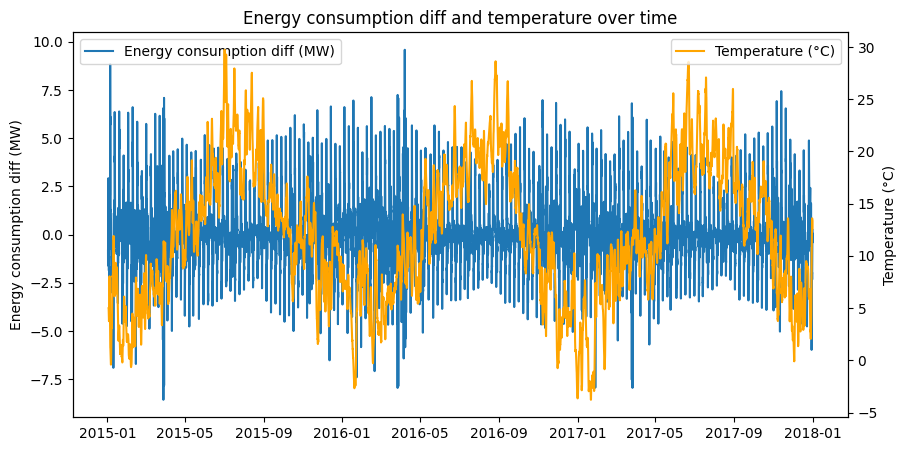
\includegraphics[width=0.82\textwidth]{meteo/overview.png}
    \caption{Overview of temperature and electricity consumption data}
\end{figure}
\end{frame}

\begin{frame}{Real Data: Météo Dataset --- Regime Detection}
Grid search on quantiser thresholds found the best parameters. The model was allowed to split on $X$ as well, but stopped before doing so, confirming that no split on $X$ is meaningful.

\begin{figure}
    \centering
    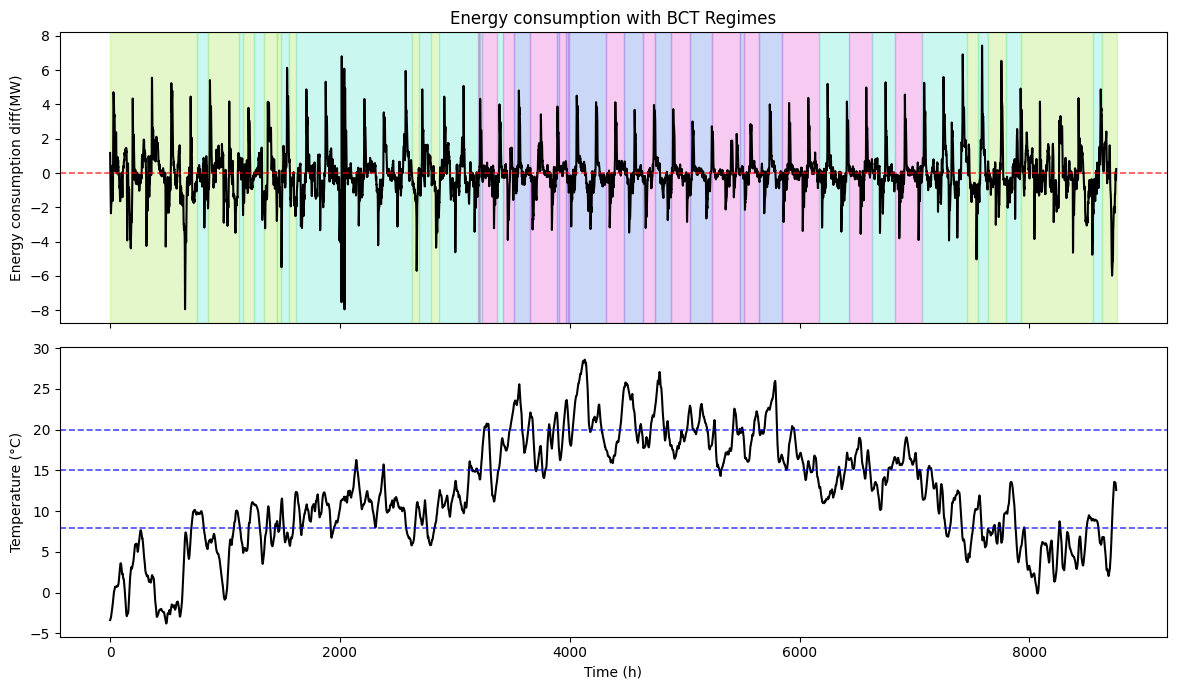
\includegraphics[width=0.82\textwidth]{meteo/meteo_regime.png}
    \caption{Observed regimes over a full year}
\end{figure}
\end{frame}

\begin{frame}{Real Data: Météo Dataset --- Fitted Tree}
\begin{figure}
    \centering
    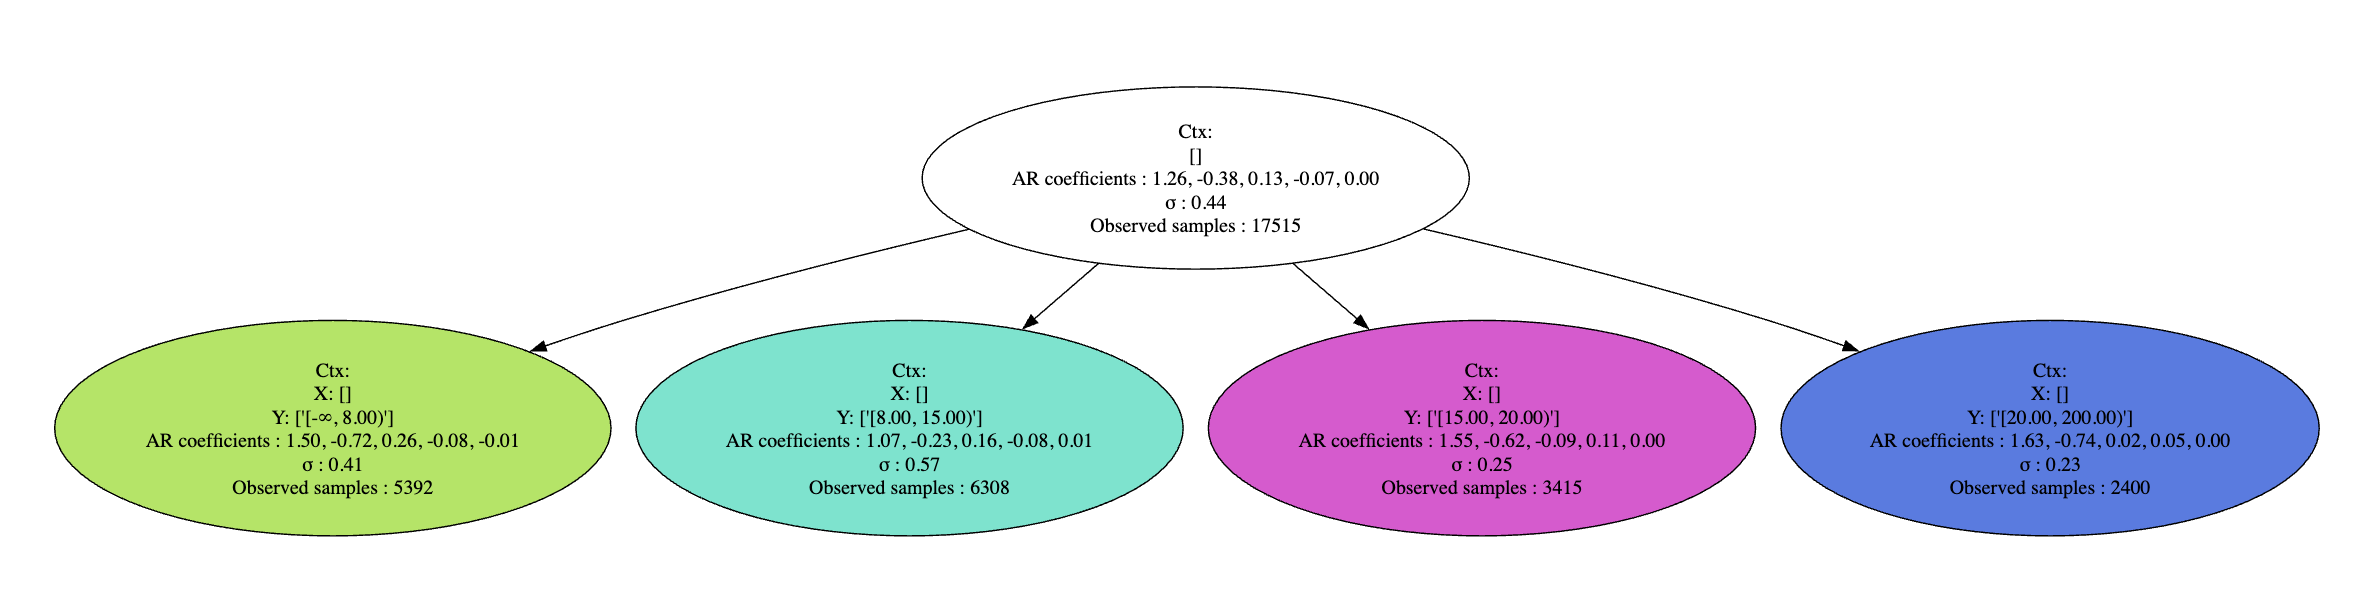
\includegraphics[width=0.75\textwidth]{meteo/meteo_tree.png}
    \caption{BCT-AR bivariate tree with identified regimes}
\end{figure}
For high and low temperatures, similar models emerge (air-conditioning and heating produce the same behaviour).
\end{frame}

\begin{frame}{Real Data: Météo Dataset --- Results}
\begin{table}[h]
\centering
\begin{tabular}{lcc}
\toprule
Model & MSE & MAE \\
\midrule
Baseline (lag 1) & 0.17269 & 0.22894 \\
AR(4) & 0.17923 & 0.21099 \\
\textbf{CTW (BCT-AR bivariate)} & \textbf{0.13664} & \textbf{0.20729} \\
\bottomrule
\end{tabular}
\caption{1-step forecasting results on Météo dataset}
\end{table}

BCT-AR bivariate achieves the lowest MSE and MAE, outperforming both the naive baseline and AR(4).
\end{frame}

%--- Real datasets: Arrhythmia
\begin{frame}{Real Data: Arrhythmia Dataset --- Overview}
\begin{itemize}
    \item Two ECG signals: \textbf{MLII} (classic ECG lead: potential difference between right arm and left leg; very sharp peaks) and \textbf{V5} (lateral view of the heart; slightly different waveform).
    \item Both measure cardiac electrical activity from two different angles.
\end{itemize}

\begin{figure}
    \centering
    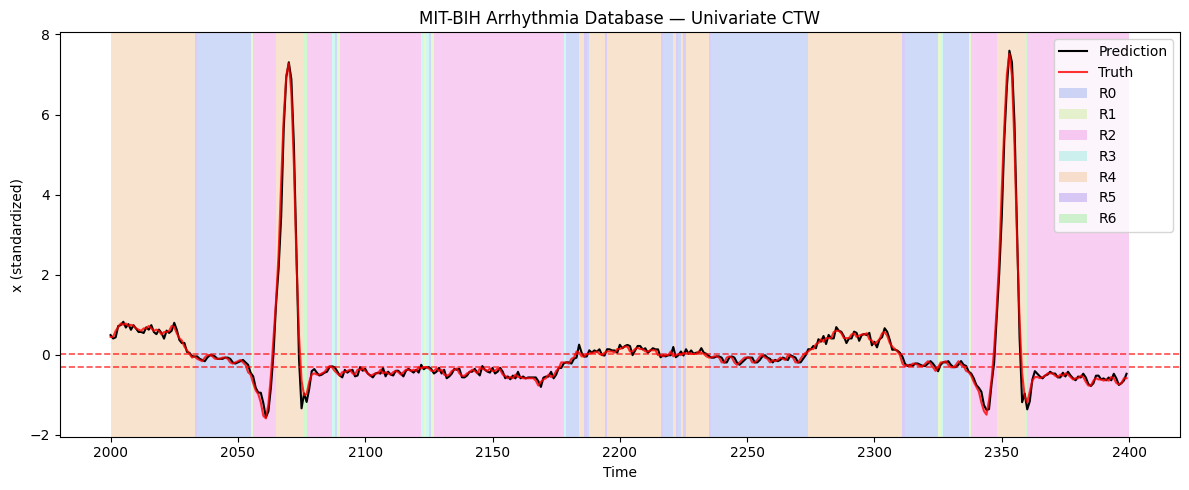
\includegraphics[width=0.82\textwidth]{arythmetia/arrhythmia_uni.png}
    \caption{Arrhythmia dataset: true vs predicted series (univariate model)}
\end{figure}
\end{frame}

\begin{frame}{Real Data: Arrhythmia Dataset --- Bivariate Results}
\begin{figure}
    \centering
    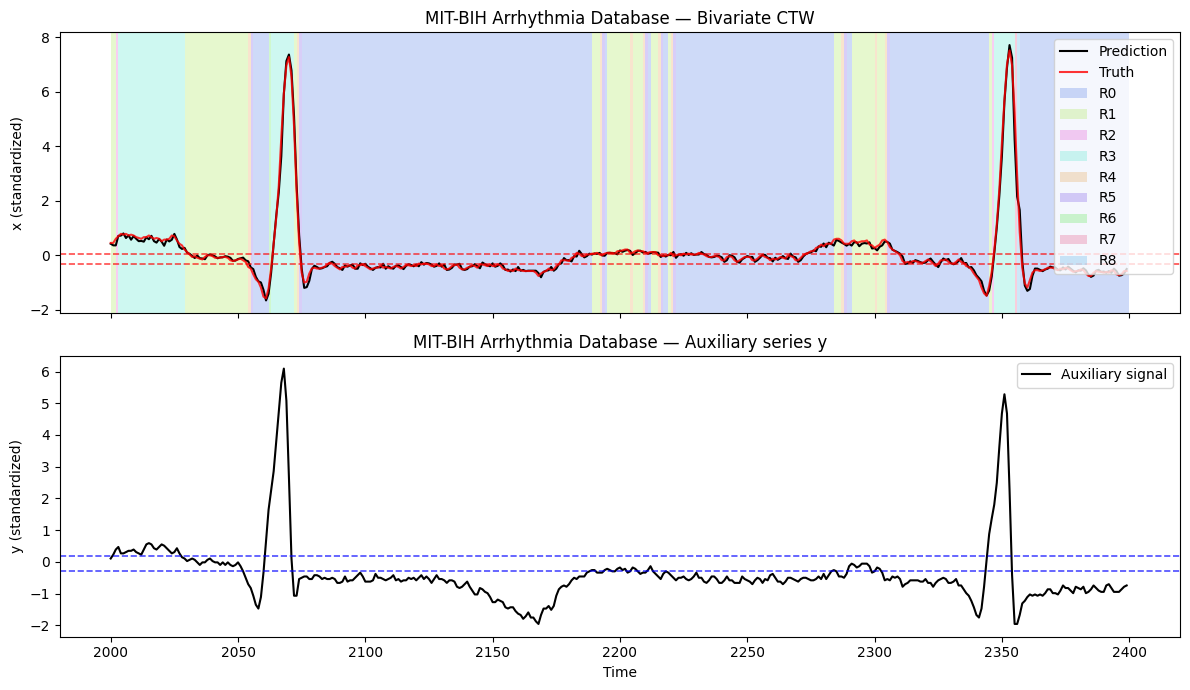
\includegraphics[width=0.82\textwidth]{arythmetia/arythmetia_bi.png}
    \caption{True vs predicted series (bivariate model)}
\end{figure}
The bivariate model shows very similar regime zones to the univariate, with a few exceptions where instabilities are resolved.
\end{frame}

\begin{frame}{Real Data: Arrhythmia Dataset --- Quantitative Results}
\small
\begin{table}[h]
\centering
\begin{tabular}{lcccc}
\toprule
Model & MSE ($k=1$) & MAE ($k=1$) & MSE ($k=5$) & MAE ($k=5$) \\
\midrule
Baseline lag1 & 0.100979 & 0.119317 & 0.856994 & 0.249120 \\
AR(2) & 0.019845 & 0.091185 & 0.170700 & 0.255355 \\
Univariate BCT-AR & 0.016130 & 0.080814 & 0.094927 & 0.167314 \\
\textbf{Bivariate BCT-AR} & \textbf{0.011590} & \textbf{0.074459} & 0.296630 & \textbf{0.200757} \\
\bottomrule
\end{tabular}
\caption{Forecasting results on Arrhythmia dataset}
\end{table}
\normalsize

The bivariate model achieves the best 1-step MSE and MAE. At horizon $k=5$, the univariate model is stronger on MSE, while bivariate leads on MAE.
\end{frame}

%--- Real datasets: PPG
\begin{frame}{Real Data: PPG Dataset --- Overview and Univariate Results}
\begin{itemize}
    \item Patients in intensive care. \textbf{X}: PPG signal (variation in blood volume in micro-vessels driven by each heartbeat). \textbf{Y}: patient respiration.
    \item Respiration modifies thoracic pressure, cardiac output and therefore PPG.
\end{itemize}

\begin{figure}
    \centering
    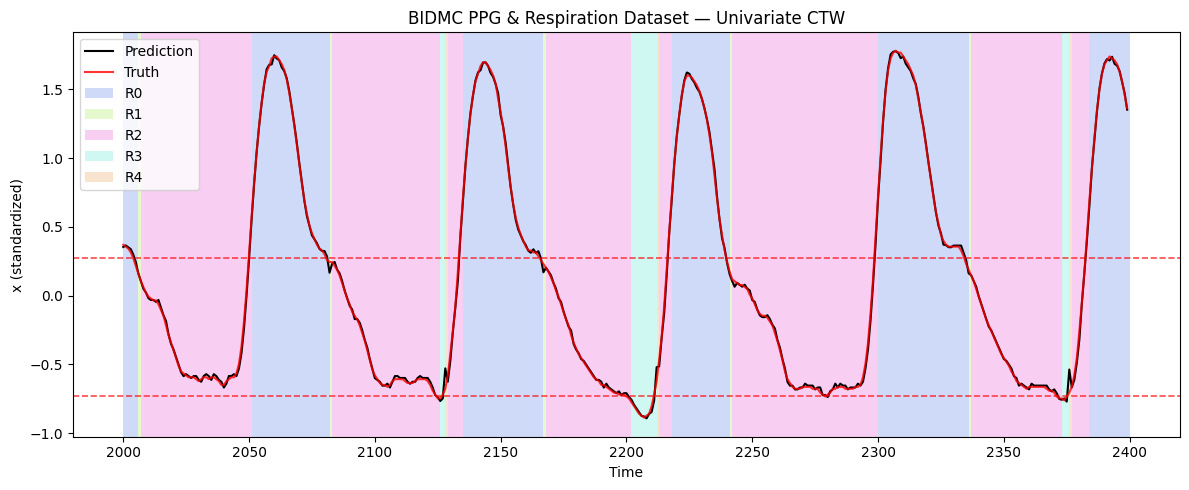
\includegraphics[width=0.82\textwidth]{PPG/uni_PPG.png}
    \caption{PPG dataset: univariate model with detected regime changes}
\end{figure}
The model correctly detects regime changes and deems them relevant.
\end{frame}

\begin{frame}{Real Data: PPG Dataset --- Results}
\small
\begin{table}[h]
\centering
\begin{tabular}{lcccc}
\toprule
Model & MSE ($k=1$) & MAE ($k=1$) & MSE ($k=5$) & MAE ($k=5$) \\
\midrule
Baseline lag1 & 0.008626 & 0.062197 & 0.088087 & 0.198508 \\
AR & 0.000396 & 0.015423 & 0.012666 & 0.071024 \\
Univariate BCT-AR & 0.000549 & 0.015877 & 0.017541 & 0.081666 \\
\textbf{Bivariate BCT-AR} & \textbf{0.000409} & \textbf{0.015379} & \textbf{0.010900} & \textbf{0.071941} \\
\bottomrule
\end{tabular}
\caption{Forecasting results on PPG dataset}
\end{table}
\normalsize

\begin{figure}
    \centering
    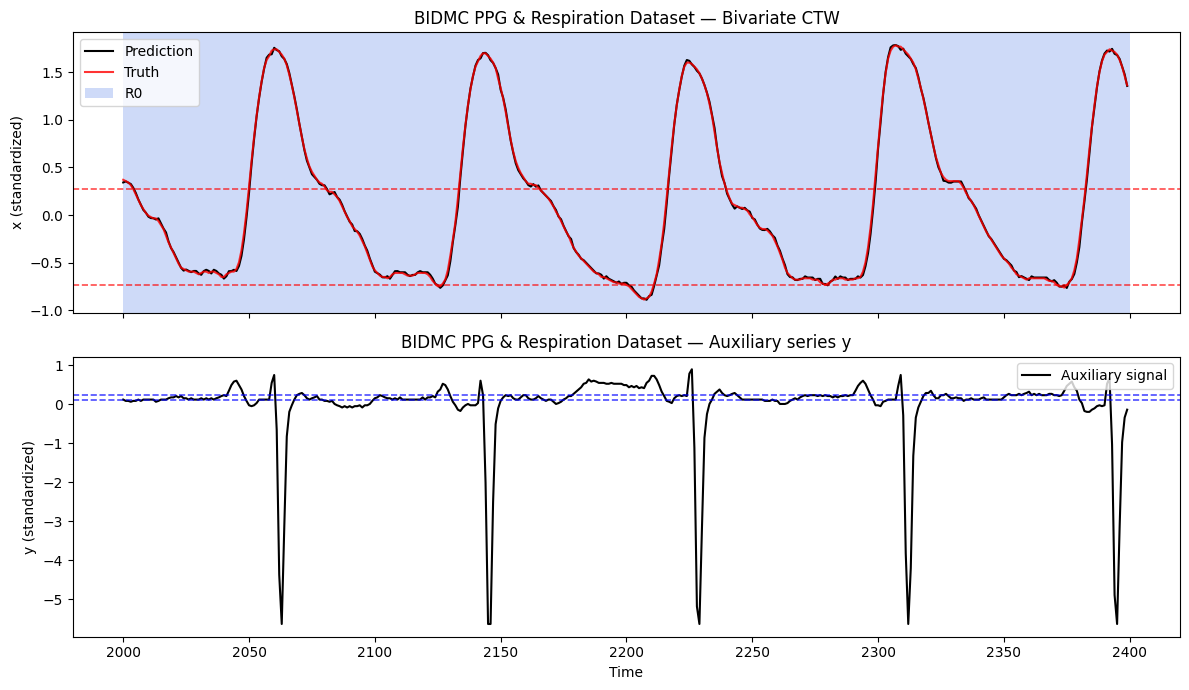
\includegraphics[width=0.6\textwidth]{PPG/bi_ppg.png}
    \caption{PPG signals $x$ and $y$ with bivariate model predictions}
\end{figure}
\end{frame}

\begin{frame}{Real Data: PPG Dataset --- Discussion}
\begin{itemize}
    \item AR is competitive here; the bivariate model gave just a simple AR tree, demonstrating that the model can stop at an AR when appropriate.
    \item Bivariate BCT-AR edges out plain AR on MSE at $k=5$ and on MAE at $k=1$, showing a marginal but consistent improvement.
\end{itemize}
\end{frame}

%--- Real datasets: Sleep Apnea
\begin{frame}{Real Data: Sleep Apnea Dataset --- Setup}
\begin{itemize}
    \item \textbf{X}: ECG time series to predict. \textbf{Y}: binary label $y \in \{0,1\}$ indicating whether the patient is experiencing sleep apnea.
    \item Goal: condition on a \emph{binary indicator} rather than a continuous series, to force regimes corresponding to apnea vs.\ no apnea.
    \item Bivariate V2 used with quantiser sequence $[1,0,0,0]$: forces quantisation on $y$ first (binary case), then the model chooses further splits.
\end{itemize}

\begin{figure}
    \centering
    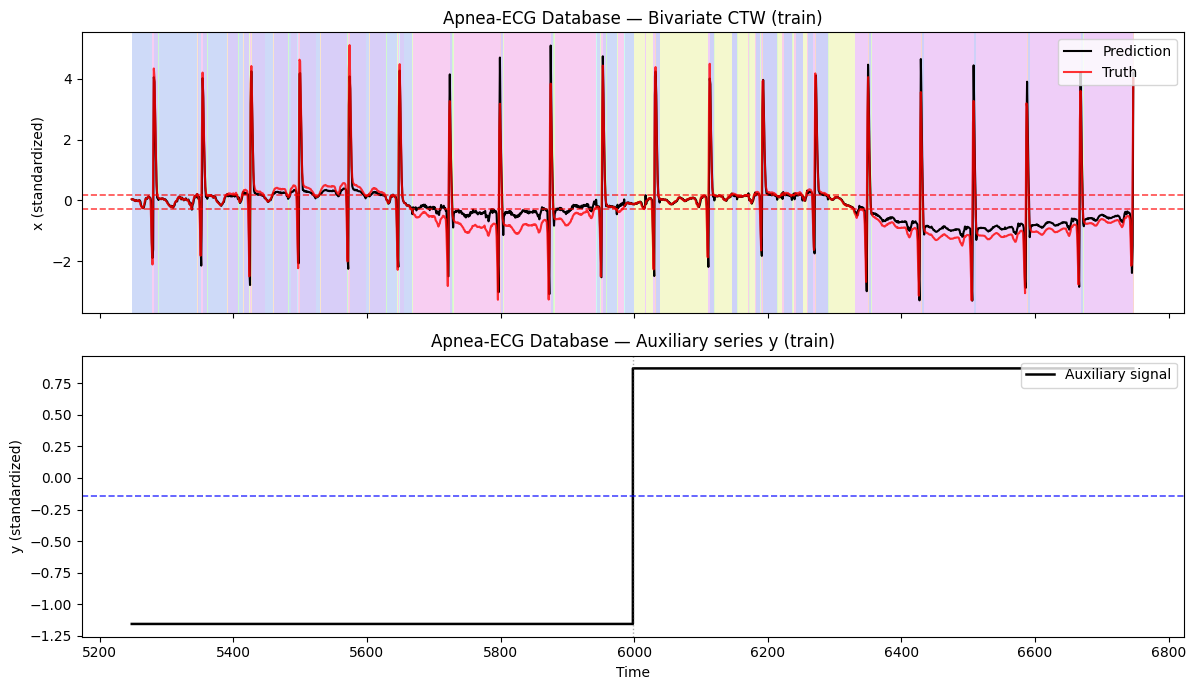
\includegraphics[width=0.78\textwidth]{apnea/bi_apnea.png}
    \caption{ECG time series: bivariate model predictions with sleep apnea label $y$}
\end{figure}
\end{frame}

\begin{frame}{Real Data: Sleep Apnea Dataset --- Fitted Tree}
\begin{figure}
    \centering
    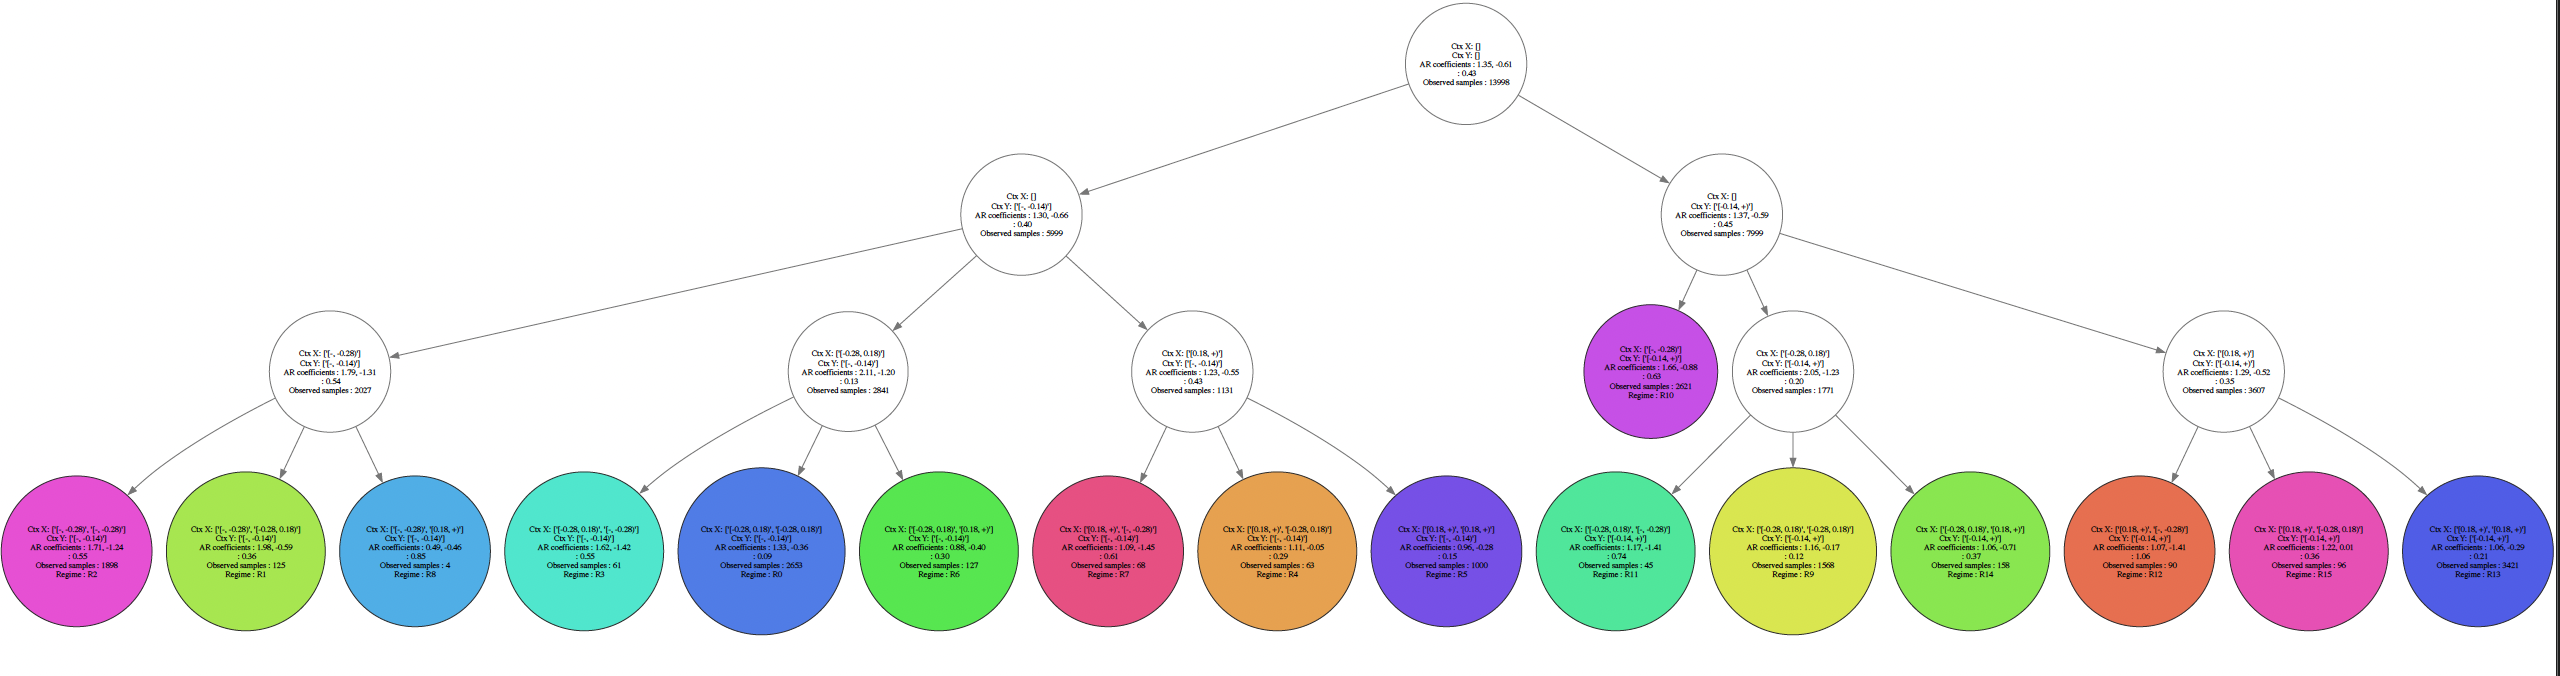
\includegraphics[width=0.80\textwidth]{apnea/tree_apnea.png}
    \caption{Bivariate BCT-AR tree (first split on $y$, the apnea indicator)}
\end{figure}
\end{frame}

\begin{frame}{Real Data: Sleep Apnea Dataset --- Quantitative Results}
\small
\begin{table}[h]
\centering
\begin{tabular}{lcccc}
\toprule
Model & MSE ($k=1$) & MAE ($k=1$) & MSE ($k=5$) & MAE ($k=5$) \\
\midrule
Baseline lag1 & 0.356286 & 0.193859 & 0.718213 & 0.246023 \\
AR & 0.181481 & 0.152179 & 0.454537 & 0.281735 \\
\textbf{Univariate BCT-AR} & \textbf{0.108016} & \textbf{0.099439} & \textbf{0.376210} & \textbf{0.221578} \\
Bivariate BCT-AR & 0.145216 & 0.123064 & 0.557362 & 0.250039 \\
\bottomrule
\end{tabular}
\caption{Forecasting results on Sleep Apnea dataset}
\end{table}
\normalsize

\begin{itemize}
    \item Here the bivariate model underperforms the univariate, but still outperforms plain AR.
    \item The binary conditioning on $y$ does not provide sufficient additional predictive structure.
\end{itemize}
\end{frame}

%%%%%%%%%%%%%%%%%%%%%%%%%%%%%%%%%%%%%%%%%%%%%%%%%%
\section{Conclusion and Perspectives}
%%%%%%%%%%%%%%%%%%%%%%%%%%%%%%%%%%%%%%%%%%%%%%%%%%

\begin{frame}{Conclusion}
\begin{block}{Main contributions}
\begin{itemize}
    \item Implemented the BCT-AR algorithm from a recent paper for time series prediction/compression.
    \item Proved the relevance of this model compared to classical autoregressive approaches.
    \item Showed that the BCT-AR models do \emph{not} work homogeneously: they can significantly outperform AR models in certain setups (e.g.\ unemployment, arrhythmia, météo).
    \item Extended the framework to a bivariate setting (two variants: V1, V2).
\end{itemize}
\end{block}

\begin{block}{Observations}
\begin{itemize}
    \item Models are highly sensitive to initialisation and hyperparameters.
    \item A rigorous method for hyperparameter selection would help stabilise training.
\end{itemize}
\end{block}
\end{frame}

\begin{frame}{Perspectives and Open Questions}
\begin{itemize}
    \item \textbf{Compression:} We did not focus much on compression. Although the link with prediction is well-documented, it would be interesting to extend the current algorithm for time series compression.

    \item \textbf{Deep learning comparison:} We compared with autoregressive models. Given the rise of deep learning, comparing BCT-AR with attention-based neural networks (e.g.\ Transformers) would be a natural next step.

    \item \textbf{Hyperparameter selection:} Developing a more principled, data-driven approach to select $\beta$, quantiser thresholds, and training window size.

    \item \textbf{Bivariate extensions:} Exploring more structured conditioning variables (e.g.\ exogenous covariates, latent states) could further improve the bivariate model's usefulness.
\end{itemize}
\end{frame}

\begin{frame}{}
\centering
\vspace{1.5cm}
{\Large \textbf{Thank you for your attention.}}\\[1.5em]
Questions?
\end{frame}

\end{document}
